\graphicspath{ {../img/} }

\section*{VirtIO}

O VirtIO é um protocolo de comunicação entre dispositivos virtuais, criado com o objetivo de definir uma API para unificar drivers e facilitar o uso e configuração desses dispositivos, 
visto que existem diversos sistemas de virtualização diferentes e cada um desses realiza a sua própria implementação.
Para alcançar tais objetivos, o virtIO define uma série de abstrações e estruturas, mas de maneira geral seus principais componentes de funcionamento são 3 (três): 
\emph{device status field}, \emph{feature bits} e uma interface chamada \emph{Virtqueue}.


O \emph{device status field} é uma sequência de bits utilizada pelo dispositivo em conjunto com o sistema operacional para realizar a inicialização do mesmo.
Os bits que podem ser setados nesse campo são: \textbf{ACKNOWLEDGE}, indicando que o dispositivo foi reconhecido, \textbf{DRIVER} para indicar que a inicialização começou, \textbf{DRIVER{\_}OK} e \textbf{FEATURES{\_}OK} para sinalizar que a comunicação está pronta para começar.
Por fim, \textbf{DEVICE{\_}NEEDS{\_}RESET} para indicar uma falha fatal do lado do dispositivo e \textbf{FAILED} pelo lado do sistema operacional.
Já o \emph{feature bits field} é utilizado para comunicar sobre quais features são suportadas pelo dispositivo e entrar em acordo com o sistema operacional sobre quais dessas serão utilizadas. Por exemplo, um dispositivo de interface de rede poderia escolher entre checksumming ou scatter-gather realizar o offload.

Por fim, temos a Virtqueue, uma interface alocada na memória do guest (dispositivo) e que realiza a comunicação entre dois grupos: front-end, onde os pedidos de I/O do processo usuário são realizados e então transferidos para o back-end, que os recebe e então executa as operações utilizando os dispositivos físicos. 

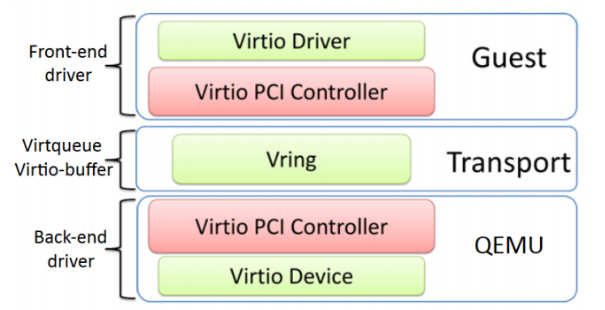
\includegraphics{virtio-arch.png}

\subsection*{Estrutura da Virtqueue}

A Virtqueue é implementada usando uma estrutura chamada \emph{Vring}, que consiste basicamente de 3 (três) partes: um array de descriptors, onde são inseridos os dados,
um \emph{available ring}, usado para a comunicação do sistema operacional com o dispositivo e um \emph{used ring}, utilizado para a comunicação no sentido do dispositivo para o sistema operacional.

Os descriptors contém um endereço físico de 64 bits de buffer junto com o seu tamanho, além de um campo para flags, que podem ser duas: uma para indicar se existe um encadeamento de buffers, permitindo o uso de memória não contígua. 
A outra flag indica o tipo do buffer, se é \emph{read-only} ou \emph{write-only}. Por fim, o campo next aponta para o próximo descriptor, se o mesmo existir. Os outros dois componentes da Virtqueue são chamados de available ring e used ring. O motivo de se utilizar essa estrutura em anéis é permitir assincronicidade, fazendo com que diversas requisições possam ser feitas sem ter que esperar por uma específica finalizar primeiro.

\begin{lstlisting}[language=C]
  struct vring_desc
  {
    __u64 addr;
    __u32 len;
    __u16 flags;
    __u16 next;
  };
\end{lstlisting}


Quando queremos realizar uma ação com o dispositivo, devemos preencher os valores desse descriptor e então adicionar o seu índice dentro de uma lista no available ring.
Dessa forma, ao notificar o sistema operacional, o mesmo irá verificar qual descriptor deve ser lido. A estrutura de um available ring possui seu índice e uma flag, onde é possível desabilitar interrupções, enquanto a constante NUM é negociada entre o dispositivo e o sistema operacional quando o mesmo é inicializado.

\begin{lstlisting}[language=C]
  struct vring_avail
  {
    __u16 ring[NUM];
    __u16 flags;
    __u16 idx;
  };
\end{lstlisting}

Ainda, temos os used rings, onde o dispositivo pode enviar algumas informações ao sistema operacional, como por exemplo indicar que uma operação foi finalizada.
Sua estrutura é muito semelhante a do available ring, com a diferença que aqui o SO tem que procurar qual descriptor realizou a notificação.

\begin{lstlisting}[language=C]
  struct vring_sed
  {
    __u16 flags;
    __u16 idx;
    __u16 avail_event;
    Elem ring[NUM];
  };

  struct Elem {
    u32 id;
    u32 len;
  }
\end{lstlisting}


Outra diferença entre o available e o used ring é que aqui, no used ring, o campo \emph{idx} indica o primeiro elemento não usado do anel.
Isso é utilizado pois dentro da estrutura 'Elem', também temos o índice do descriptor. Assim, a cada leitura realizada, o dispositivo incrementa o índice em used ring.
Dessa forma, se os índices não são iguais, significa que existe ainda dados a serem lidos. 	Tanto o sistema operacional quanto o dispositivo acompanham o estado desses anéis, garantindo que estejam falando sobre a mesma requisição.


Por fim, para indicar onde procurar na memória pelos descriptors, os dispositivos do virtIO tem um registrador chamado \emph{QueuePFN (Page Field Number)} , que contém o endereço de memória física para o qual foi mapeado. Com esse componentes, conseguimos então realizar todo o ciclo de uma requisição. Iniciamos apontando para o endereço de memória existente em QueuePFN e então, quando um descriptor for preenchido com dados, notificamos que uma requisição foi realizada através de um outro registrador, chamado \emph{QueueNotify}, escrevendo um valor qualquer no mesmo. O processo se inicia e quando o mesmo finalizar, uma interrupção externa será enviada pelo dispositivo, de forma que o sistema operacional precisa apenas verificar o used ring e obter os dados.


\subsection*{Exemplo de configuração e uso de um dispositivo}

Para iniciar o processo de uso e configuração de um dispositivo, precisamos começar lendo todo o barramento e procurar pelo chamado \emph{Magic Value}, i.e, a string 'virt'.
Neste exemplo, usando o QEMU, precisamos verificar todos os endereços entre 0x1000{\_}1000 e 0x1000{\_}8000, pois é onde os dispositivos virtios são alocados pelo QEMU.
Encontrado esse valor, podemos ler então o valor do registrador \emph{DeviceID}, que identifica o tipo de dispositivo. Nesse caso, procuramos pelo valor 2, para \emph{block devices}.
O trecho de código abaixo mostra um pedaço dessa leitura de endereços até encontrarmos o dispositivo desejado.

\begin{lstlisting}[language=C]
for addr in (MMIO_VIRTIO_START..=MMIO_VIRTIO_END).step_by(MMIO_VIRTIO_STRIDE) {
  let magicvalue;
  let device_id;
  let ptr = addr as *mut u32;

  unsafe {
    magicvalue = ptr.read_volatile();
    deviceid = ptr.add(2).read_volatile();
  }

  if MMIO_VIRTIO_MAGIC != magicvalue {
    continue;
  }
  else if 0 == deviceid {
    println!("not connected.");
  }
  else {
    match deviceid {
      2 => {
        if false == setup_block_device(ptr) {
          println!("setup failed.");
        }
        else {
          let idx = (addr - MMIO_VIRTIO_START) >> 12;
          unsafe {
            VIRTIO_DEVICES[idx] =
              Some(VirtioDevice::new_with(DeviceTypes::Block));
          }

          println!("setup succeeded!");
        }
      },
      _ => println!("unknown device type."),
    }
  }
}
\end{lstlisting}

Feito isso, começamos a configurar o dispositivo e sua comunicação com o sistema operacional. Iniciamos essa configuração setando o bit de \textbf{ACKNOWLEDGE} no device status, seguido do bit de \textbf{DRIVER}.
Além disso, precisamos entrar em acordo com o dispositivo sobre quais features serão habilitadas, através da leitura do registrador \emph{guest{\_}features} e então setando o bit de \textbf{FEATURES{\_}OK}. 
Por fim, setamos o bit de \textbf{DRIVER{\_}OK} e agora o dispositivo está conectado. O trecho de código abaixo mostra como seria esse processo para um dispositivo genérico.

\begin{lstlisting}[language=C]
  // Reseta o dispositivo e pega o status bit
  ptr.add(MmioOffsets::Status.scale32()).write_volatile(0); 
  let mut status_bits = StatusField::Acknowledge.val32();

  // Seta o ACKNOWLEDGE e o DRIVER no status bit
  ptr.add(MmioOffsets::Status.scale32()).write_volatile(status_bits);
  status_bits |= StatusField::DriverOk.val32();
  ptr.add(MmioOffsets::Status.scale32()).write_volatile(status_bits);

  // Seta o FEATURES{\_}OK no status bit
  status_bits |= StatusField::FeaturesOk.val32();
  ptr.add(MmioOffsets::Status.scale32()).write_volatile(status_bits);

  // Seta o DRIVER{\_}OK no status bit e o dispositivo está conectado
  status_bits |= StatusField::DriverOk.val32();
  ptr.add(MmioOffsets::Status.scale32()).write_volatile(status_bits);
\end{lstlisting}

O VirtIO define uma série de protocolos para cada tipo de dispositivo quando vamos fazer uma requisição, então precisamos seguir o definido para dispositivos do tipo block.
Sendo assim, usaremos 3 (três) descriptors nesse processo: uma para o header, buffer e status.
O do header é responsável por dizer para o dispositivo se o sistema operacional quer escrever ou ler e o endereço onde essa ação deve ocorrer.
O buffer, se for de leitura, irá escrever seu valor na memória, caso seja escrita, o dispositivo irá ler o endereço na memória.
Por fim, o status field guarda o resultado da requisição, que pode ter 3 (três) valores: 0 - success, 1 - failure ou 2 - unsupported operation.


Para realizar a requisição, pegamos os três descriptors que precisamos, inserimos os dados de header, buffer e status e então escrevemos o valor 0 dentro do registrador queue{\_}notify para avisar ao dispositivo que ele deve iniciar a trabalhar na requisição.
Ao finalizar a execução, o dispositivo então emite uma interrupção e recebemos de volta um used ring, o qual contém um id para identificar o descriptor usado. Isto se deve pois as requisições podem 
acabar numa ordem diferente do que foram enviadas, o que faz com que não tenhamos garantia de que é o mesmo descriptor e torna necessário que isso seja checado.
Por fim, validado o descriptor e recebida a resposta, é possível liberar a memória da heap que foi alocada no ínicio da requisição e finalizar a mesma.

\begin{lstlisting}[language=C]
  
\end{lstlisting}